\subsection{Completed-round rates}\label{app:subsequent-rates}

\begin{figure*}[!t]
  \centering
  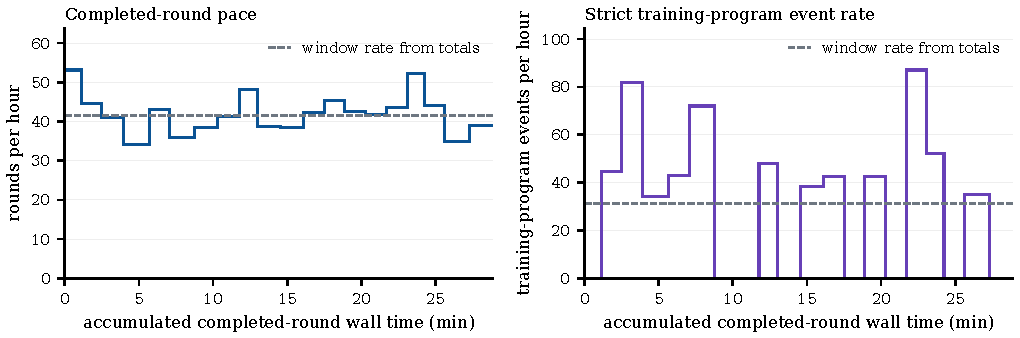
\includegraphics[width=\linewidth,height=1.08in,keepaspectratio]{figures/fig_fw_subsequent_rates.pdf}
  \caption{\textbf{Work and training-program event rates in the subsequent window.}
  Left: completed rounds per hour. Right: strict training-program incumbent
  events per hour. Each step is an average over one completed round's logged
  wall time; dashed lines are rates from whole-window totals. Both panels
  use the same 20 summaries as \cref{fig:fw-subsequent-window}, with no new
  observations. Program events do not count adapter admissions.}
  \label{fig:fw-subsequent-rates}
\end{figure*}

\begin{figure*}[!t]
  \centering
  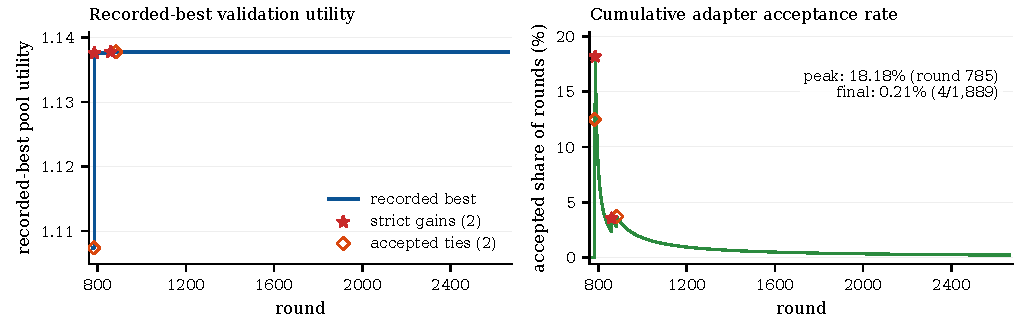
\includegraphics[width=\linewidth,height=1.08in,keepaspectratio]{figures/fig_fw_acceptance_over_rounds.pdf}
  \caption{\textbf{Recorded-best validation utility and cumulative adapter acceptance rate over rounds.}
  Both panels use the same \num{1889} consecutive admission rounds, 775--2663, as
  \cref{fig:fw-validation}, adding no observations. Left: post-decision
  recorded-best validation pool utility, with stars at strict gains (rounds
  785 and 859) and hollow diamonds at accepted ties (rounds 782 and 882).
  Right: cumulative accepted share of elapsed rounds (\%), which peaks at
  18.18\% at round 785 and falls to 0.21\% ($4/\num{1889}$) across the
  subsequent \num{1781} rejected rounds. Scope: \cref{sec:method-status}.}
  \label{fig:fw-acceptance-over-rounds}
\end{figure*}

\Cref{fig:fw-subsequent-rates} reuses the 20 summaries from rounds
2508--2527 in \cref{app:subsequent-window}. Each step divides one completed
round, or its strict training-program event count, by that round's logged
wall time. Its width is the corresponding duration. Dashed lines divide
the window's total work or events by its total time; they do not average
the per-round rates.

Time includes logged qualification waits and omits gaps outside completed
rounds. None records an adapter admission. Scope: \cref{sec:method-status}.
